\documentclass[10pt]{report}
\usepackage[utf8]{inputenc}
\usepackage[T1]{fontenc}
\usepackage[french]{babel}
\usepackage{array}
\usepackage{color}
\usepackage{hyperref}
\usepackage{amssymb}
\usepackage{tikz}
\usepackage{stmaryrd}
\usepackage{graphicx}

\usetikzlibrary{arrows}

\title{Intelligence Artificielle\\Réseaux de neurones\\Perceptron et perceptron multi-couches avec Neuroph}
\date{S6 Printemps 2017}
\author{MEYER Cyril}

\begin{document}
\selectlanguage{french}

\maketitle
\newpage
\tableofcontents
\newpage

\chapter{Apprentissage d'une fonction}
\section{Fonctions booléennes}
\subsection{"Et" logique}
La table de vérité du "Et" logique est la suivante :\\

\begin{center}
\begin{tabular}{|c|c|c|}
	\hline
	a & b & a $\land$ b \\
	\hline
	0 & 0 & 0 \\
	\hline
	0 & 1 & 0 \\
	\hline
	1 & 0 & 0 \\
	\hline
	1 & 1 & 1 \\
	\hline
\end{tabular}
\end{center}

Nous créons un percetron mono-couche avec 2 neurones d'entrée et 1 neurone de sortie. Le dataset utilisé est la table logique de la fonction et (cf dataset\_AND.csv).\\


\begin{center}
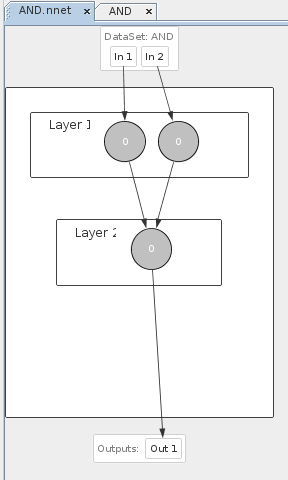
\includegraphics[height=300px]{img/AND_NN.png}\\
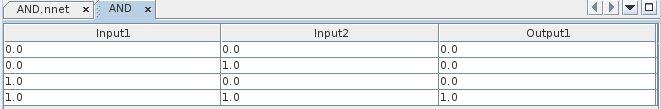
\includegraphics[width=400px]{img/AND_TS.png}\\
\end{center}

Configuration d'entraînement :\\
\begin{tabular}{|l|c|}
	\hline
	Max Error & 0.01 \\
	\hline
	Learning Rate & 0.2 \\
	\hline
	Momentum & 0.7 \\
	\hline
\end{tabular}

Résultats (2 test) :\\
\begin{center}
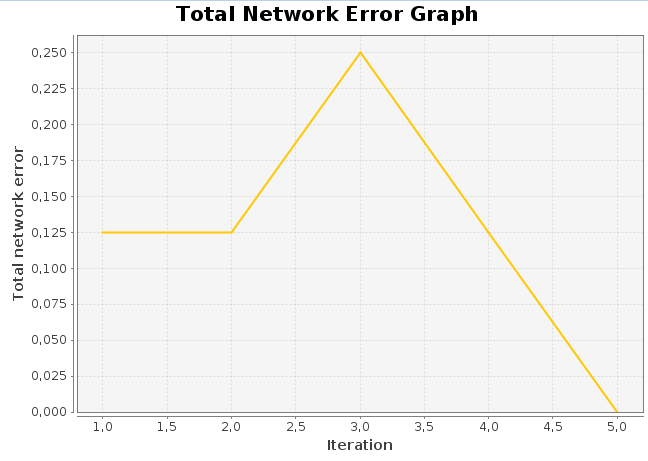
\includegraphics[height=200px]{img/AND_EG_1.png}\\
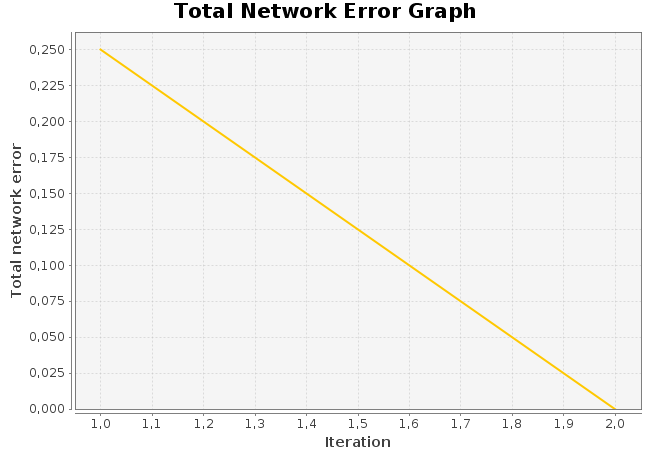
\includegraphics[height=200px]{img/AND_EG_2.png}\\
\end{center}

La courbe tend très rapidement vers la solution parfaite (taux d'erreur de 0.0). On peut tout de même remarqué que dans lors du premier essai, le réseaux s'est dégradé lors de la troisième itération.\\

Configuration d'entraînement :\\
\begin{tabular}{|l|c|}
	\hline
	Max Error & 0.01 \\
	\hline
	Learning Rate & 0.1 \\
	\hline
	Momentum & 0.7 \\
	\hline
\end{tabular}

Résultats :\\
\begin{center}
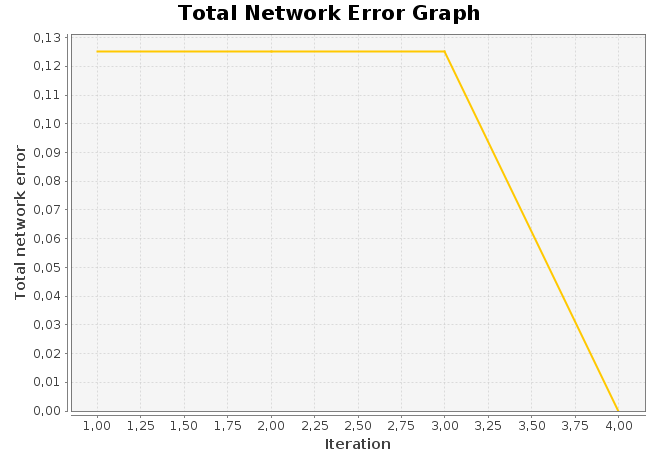
\includegraphics[height=200px]{img/AND_EG_3.png}\\
\end{center}

Configuration d'entraînement :\\
\begin{tabular}{|l|c|}
	\hline
	Max Error & 0.01 \\
	\hline
	Learning Rate & 1 \\
	\hline
	Momentum & 0.7 \\
	\hline
\end{tabular}

Résultats :\\
\begin{center}
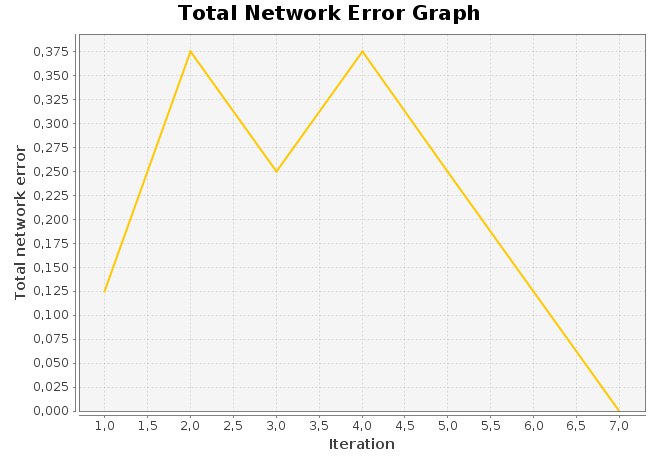
\includegraphics[height=200px]{img/AND_EG_4.png}\\
\end{center}

On ce rend compte que le pas d'apprentissage importe beaucoup sur les résultats du réseau.
 
\subsection{"Équivalence" logique}
La table de vérité de l'equivalence logique est la suivante :\\

\begin{center}
\begin{tabular}{|c|c|c|}
	\hline
	a & b & a $\iff$ b \\
	\hline
	0 & 0 & 1 \\
	\hline
	0 & 1 & 0 \\
	\hline
	1 & 0 & 0 \\
	\hline
	1 & 1 & 1 \\
	\hline
\end{tabular}
\end{center}

Nous créons un percetron mono-couche avec 2 neurones d'entrée et 1 neurone de sortie. Le dataset utilisé est la table logique de la fonction d'équivalence (cf dataset\_EQ.csv).\\

Configuration d'entraînement :\\
\begin{tabular}{|l|c|}
	\hline
	Max Error & 0.01 \\
	\hline
	Limite Max Iterations & 1000 \\
	\hline
	Learning Rate & 0.2 \\
	\hline
	Momentum & 0.7 \\
	\hline
\end{tabular}

Résultats :\\
\begin{center}
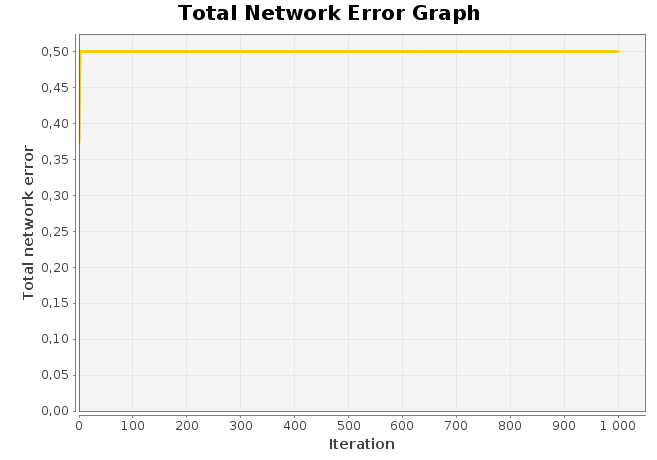
\includegraphics[height=200px]{img/EQ_EG_1.png}\\
\end{center}

L'apprentissage ne permet pas de converger. Les pas d'apprentissage différents ne changerais rien, un perceptron mono-couche ne peut pas résoudre ce genre de problème car ce n'est pas linéairement séparable.\\

Nous créons un percetron multi-couche (1 couche cachée de 3 noeuds) avec 2 neurones d'entrée et 1 neurone de sortie. Le dataset utilisé est la table logique de la fonction d'équivalence (cf dataset\_EQ.csv).\\

Configuration d'entraînement :\\
\begin{tabular}{|l|c|}
	\hline
	Max Error & 0.01 \\
	\hline
	Learning Rate & 0.2 \\
	\hline
	Momentum & 0.7 \\
	\hline
\end{tabular}

Résultats (2 test) :\\
\begin{center}
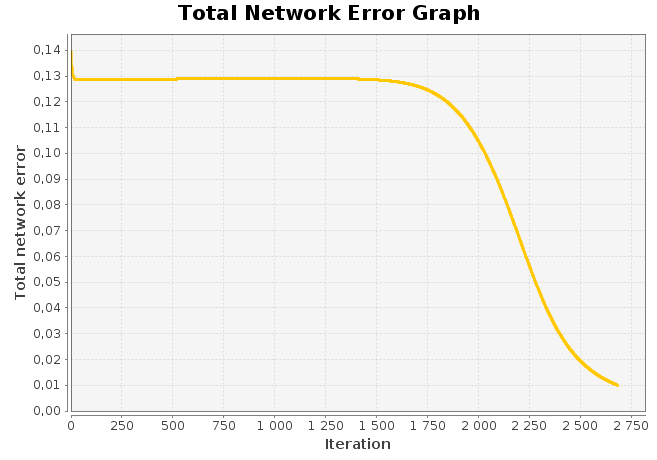
\includegraphics[height=200px]{img/EQ_EG_2.png}\\
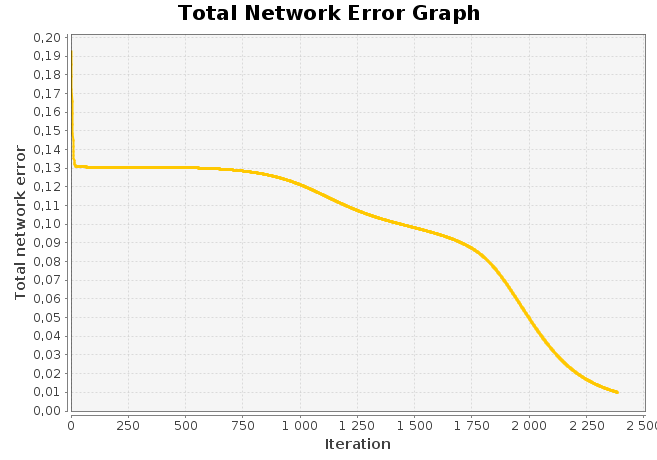
\includegraphics[height=200px]{img/EQ_EG_3.png}\\
\end{center}

La courbe d'apprentissage stagne un bon moment avant de tendre plus rapidement vers la solution.

\subsubsection{Influence des paramètres}

Lorsque ce ne sera pas précisé, la configuration d'entraînement sera la suivante :\\
\begin{tabular}{|l|c|}
	\hline
	Max Error & 0.01 \\
	\hline
	Limite Max Iterations & 5000 \\
	\hline
	Learning Rate & 0.2 \\
	\hline
	Momentum & 0.7 \\
	\hline
\end{tabular}

\paragraph{1. Nombre de couche}

Résultats (2 couches de 3 noeuds) :\\
\begin{center}
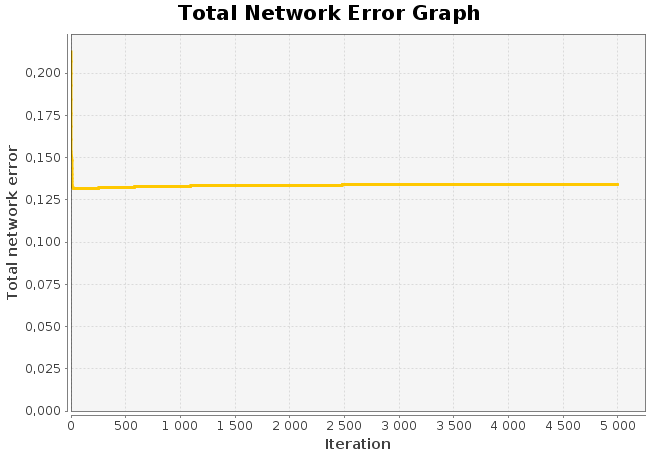
\includegraphics[height=200px]{img/EQ_EG_4.png}\\
\end{center}

Résultats (3 couches de 3 noeuds) :\\
\begin{center}
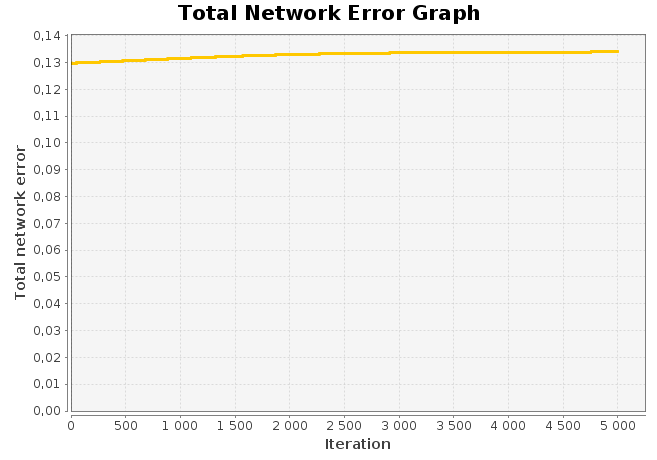
\includegraphics[height=200px]{img/EQ_EG_5.png}\\
\end{center}

Conclusion : Ajouté des couches n'améliore pas les résultats.

\paragraph{2. Nombre de noeuds}

Résultats (1 couches de 12 noeuds) :\\
\begin{center}
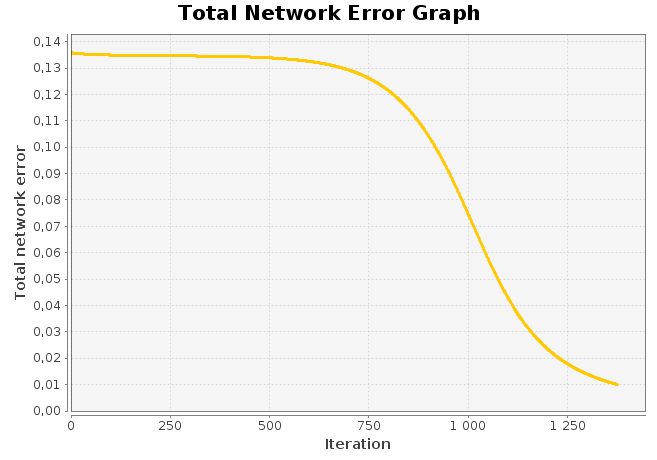
\includegraphics[height=200px]{img/EQ_EG_6.png}\\
\end{center}

Résultats (1 couches de 24 noeuds) :\\
\begin{center}
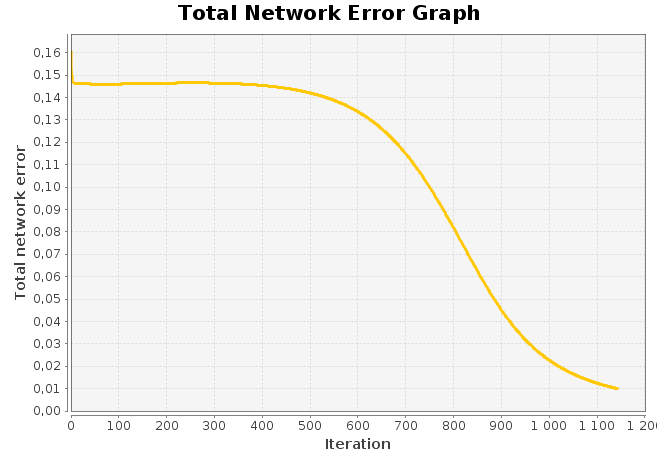
\includegraphics[height=200px]{img/EQ_EG_7.png}\\
\end{center}

Conclusion : Ajouté des noeuds permet de converger plus rapidement vers le résultat.

\paragraph{3. Fonction d'activation Tanh}

Résultats  :\\
\begin{center}
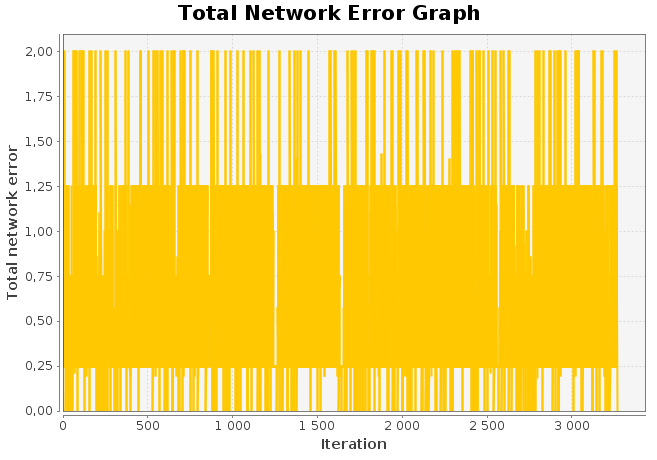
\includegraphics[height=200px]{img/EQ_EG_8.png}\\
\end{center}

Résultats (Pas d'apprentissage de 0.01) :\\
\begin{center}
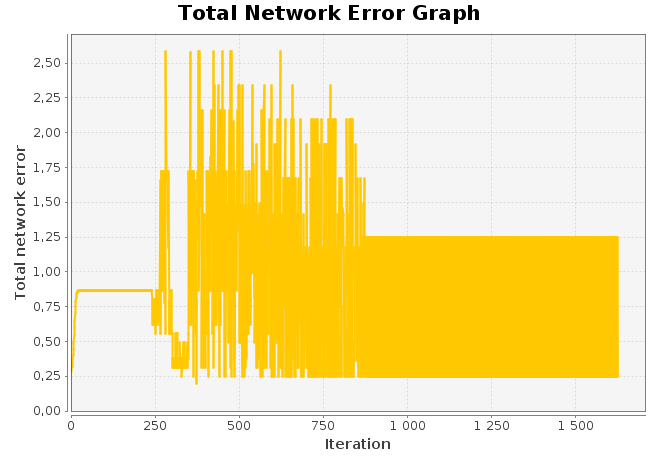
\includegraphics[height=200px]{img/EQ_EG_9.png}\\
\end{center}

Conclusion : La fonction Tanh crée des variation de l'erreur beaucoup plus grande, cela n'améliore pas la convergence.

\paragraph{4. Pas d'apprentissage}

Résultats (Pas d'apprentissage de 1) :\\
\begin{center}
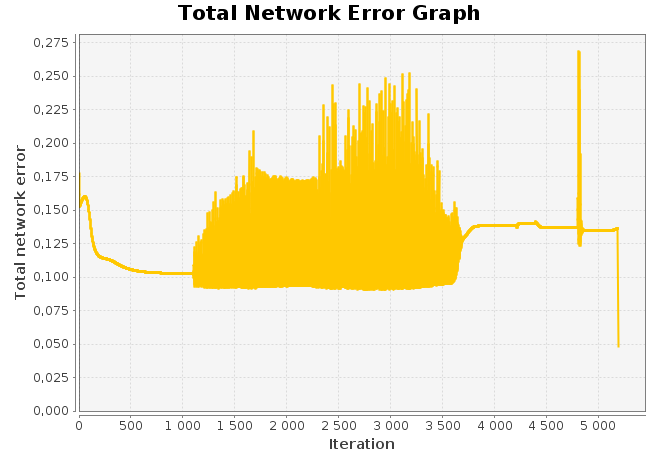
\includegraphics[height=200px]{img/EQ_EG_10.png}\\
\end{center}

Résultats (Pas d'apprentissage de 0.01) :\\
\begin{center}
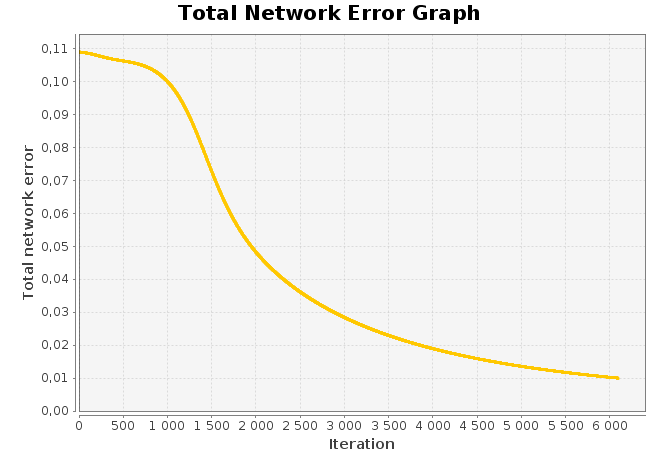
\includegraphics[height=200px]{img/EQ_EG_11.png}\\
\end{center}

Conclusion : Un pas d'apprentissage plus petit permet de converger plus précisément vers le résultat.

\paragraph{Conclusion}
En utilisant les conclusions précédentes, on peut se demander si un pas d'apprentissage petit ainsi qu'un nombre de noeuds supplémentaire améliorerais les résultats.\\
Résultat d'un test avec les paramètres suivants :\\

\begin{tabular}{|l|c|}
	\hline
	Max Error & 0.01 \\
	\hline
	Learning Rate & 0.01 \\
	\hline
	Momentum & 0.7 \\
	\hline
	Couches & 1 \\
	\hline
	Noeuds & 20 \\
	\hline
\end{tabular}

\begin{center}
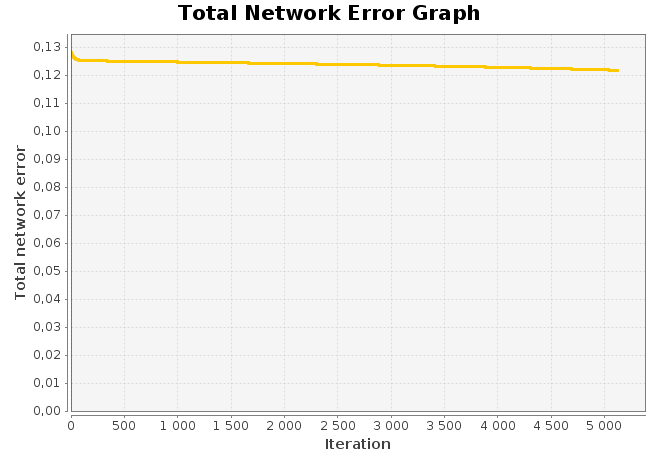
\includegraphics[height=200px]{img/EQ_EG_12.png}\\
\end{center}

Conclusion : Les résultats ne sont pas positifs.

\section{Fonctions simples}
\subsection{Fonction $f(x)=x^2$}

Je commence tout d'abord en crée plusieurs réseaux de neurones multi-couches, le problème $f(x)=x^2$ est un problème qui n'est pas linéairement séparable, donc impossible a résoudre avec un perceptron mono-couche.

J'ai choisis de tester différent dataset. Respectivement, 21, 101, 302 et 704 exemples. Les dataset sont disponible sous les noms : "dataset\_SQUARE\_xxx"
Ces dataset sont crée avec le programme "squareDataset".

Ces premiers tests me permettent de comprendre quels réseaux et quels dataset choisir pour les tests suivants qui seront plus précis.

Le premier dataset (21) est utilisé pour tester les différence entre les différentes architectures de réseau.

\begin{center}

\begin{tabular}{|l|c|}
	\hline
	Max Error & 0.01 \\
	\hline
	Learning Rate & 0.2 \\
	\hline
	Momentum & 0.7 \\
	\hline
\end{tabular}

Perceptron multicouche : 1 couche de 8 noeuds.\\
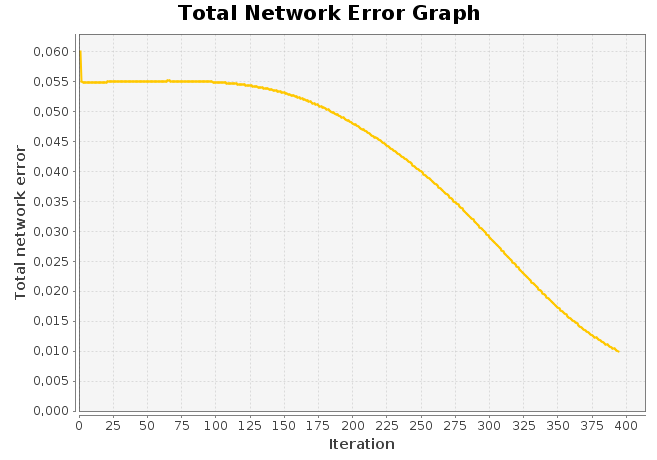
\includegraphics[height=200px]{img/SQUARE_8_21.png}\\
Perceptron multicouche : 1 couche de 16 noeuds.\\
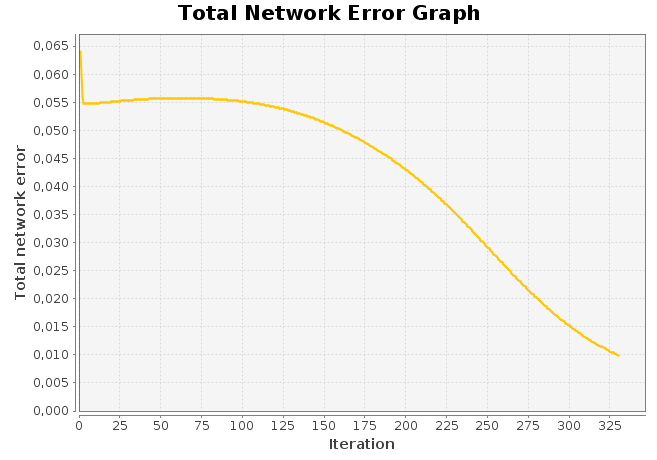
\includegraphics[height=200px]{img/SQUARE_16_21.png}\\
Perceptron multicouche : 1 couche de 32 noeuds.\\
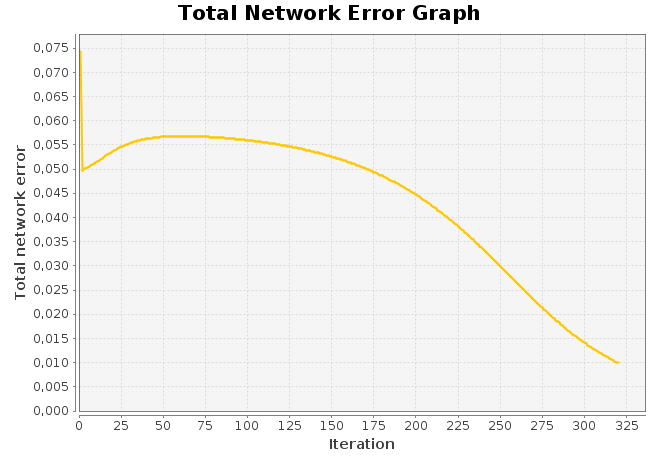
\includegraphics[height=200px]{img/SQUARE_32_21.png}\\
Perceptron multicouche : 2 couche de 8 noeuds.\\
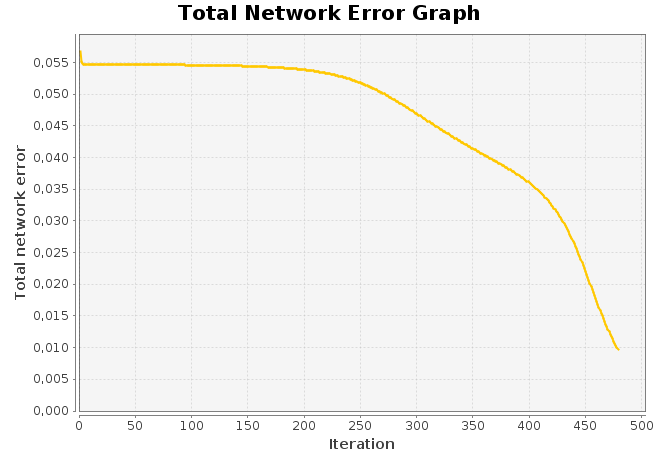
\includegraphics[height=200px]{img/SQUARE_8_8_21.png}\\
Perceptron multicouche : 2 couche de 16 noeuds.\\
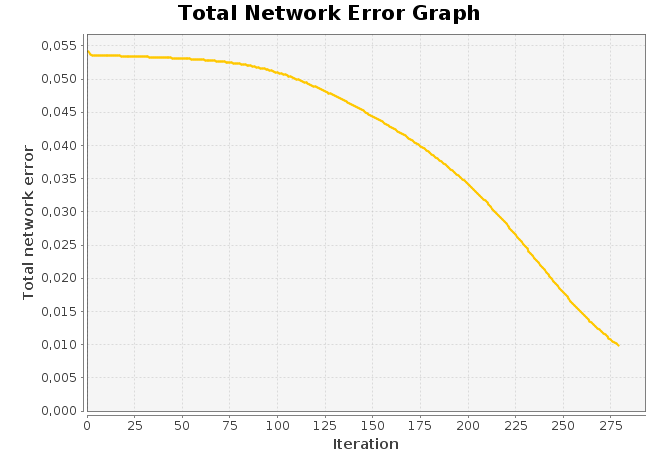
\includegraphics[height=200px]{img/SQUARE_16_16_21.png}\\
Perceptron multicouche : 2 couche de 32 noeuds.\\
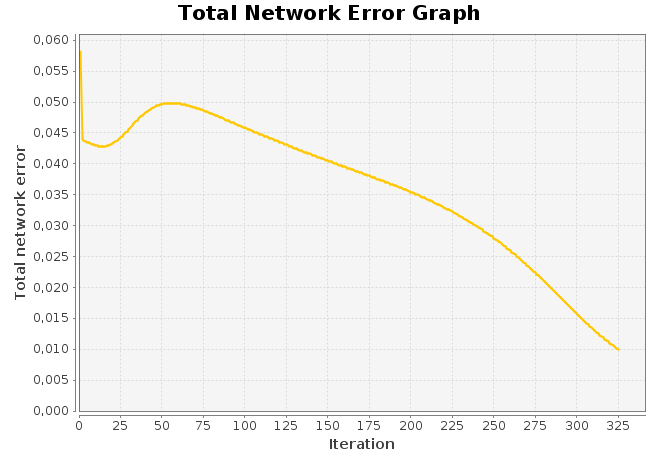
\includegraphics[height=200px]{img/SQUARE_32_32_21.png}\\
Perceptron multicouche : 3 couche de 16 noeuds.\\
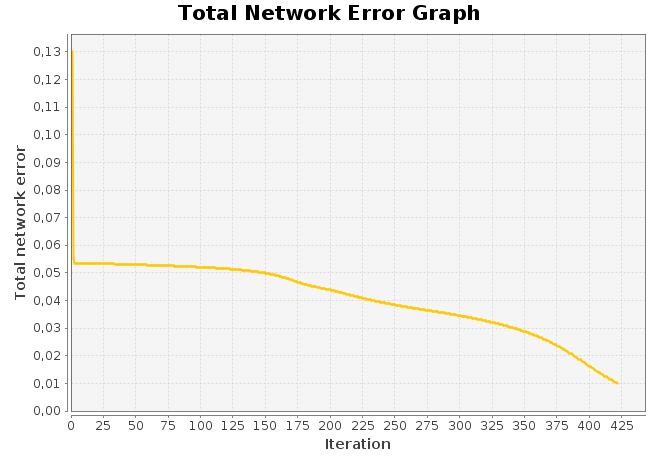
\includegraphics[height=200px]{img/SQUARE_16_16_16_21.png}\\
\end{center}

Le second dataset (101) est utilisé pour choisir parmi les meilleurs résultats précédents.

\begin{center}

\begin{tabular}{|l|c|}
	\hline
	Max Error & 0.001 \\
	\hline
	Learning Rate & 0.2 \\
	\hline
	Momentum & 0.7 \\
	\hline
\end{tabular}

Perceptron multicouche : 1 couche de 8 noeuds.\\
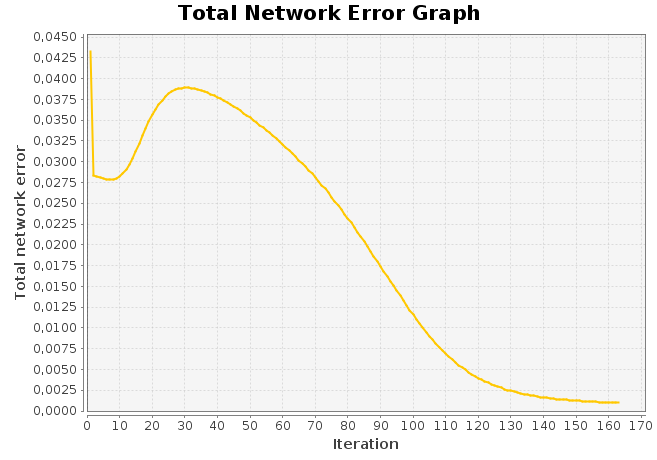
\includegraphics[height=200px]{img/SQUARE_8_101.png}\\
Perceptron multicouche : 1 couche de 16 noeuds.\\
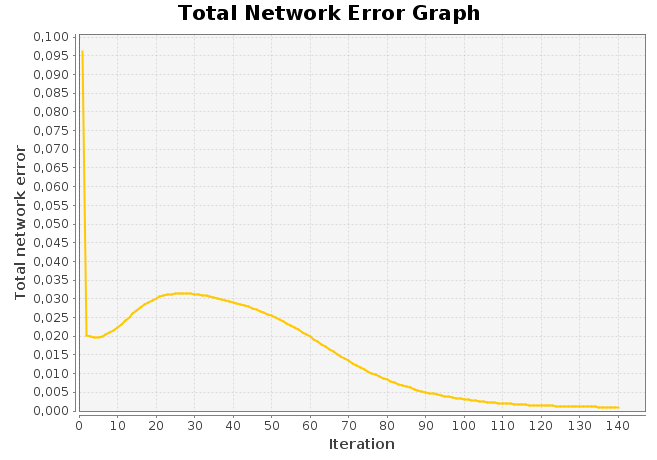
\includegraphics[height=200px]{img/SQUARE_16_101.png}\\
Perceptron multicouche : 2 couche de 16 noeuds.\\
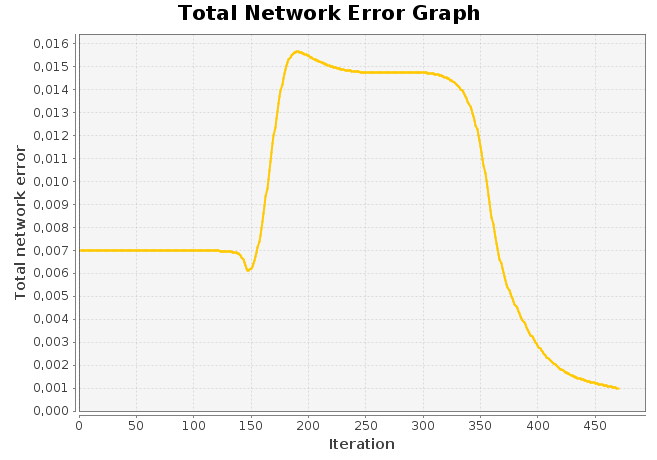
\includegraphics[height=200px]{img/SQUARE_16_16_101.png}\\
\end{center}


Le troisième dataset (302) est utilisé pour choisir parmi les meilleurs résultats précédents.

\begin{center}

\begin{tabular}{|l|c|}
	\hline
	Max Error & 0.1 \\
	\hline
	Learning Rate & 0.2 \\
	\hline
	Momentum & 0.7 \\
	\hline
\end{tabular}

Perceptron multicouche : 1 couche de 8 noeuds.\\
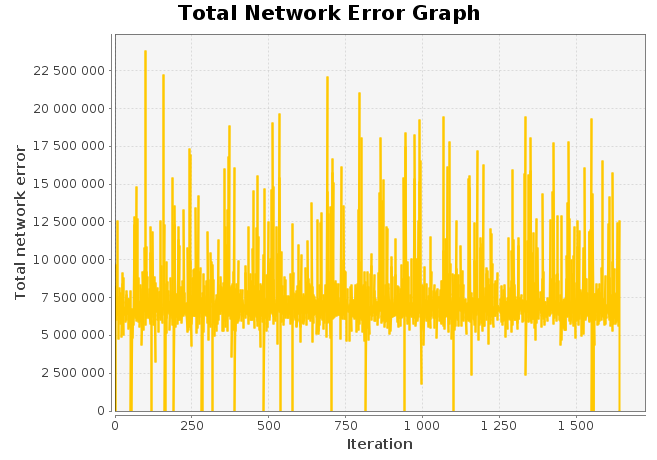
\includegraphics[height=200px]{img/SQUARE_8_302.png}\\
Perceptron multicouche : 1 couche de 16 noeuds.\\
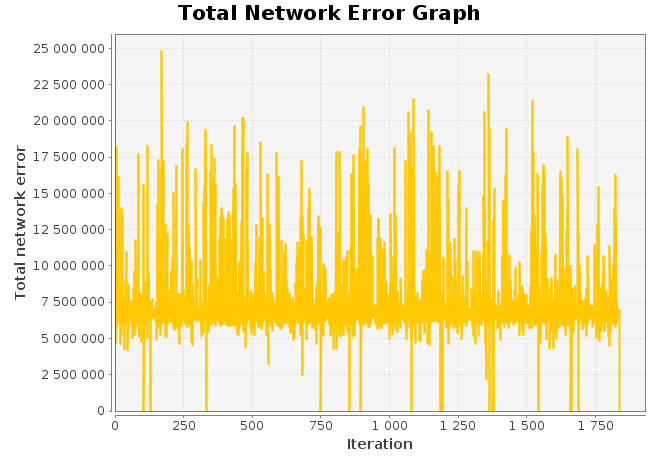
\includegraphics[height=200px]{img/SQUARE_16_302.png}\\
\end{center}

Aucun des réseau ne converge.

Un dernier essai avec le dernier dataset (704) :

\begin{center}

\begin{tabular}{|l|c|}
	\hline
	Max Error & 1000 \\
	\hline
	Learning Rate & 0.2 \\
	\hline
	Momentum & 0.7 \\
	\hline
\end{tabular}

Perceptron multicouche : 1 couche de 16 noeuds.\\
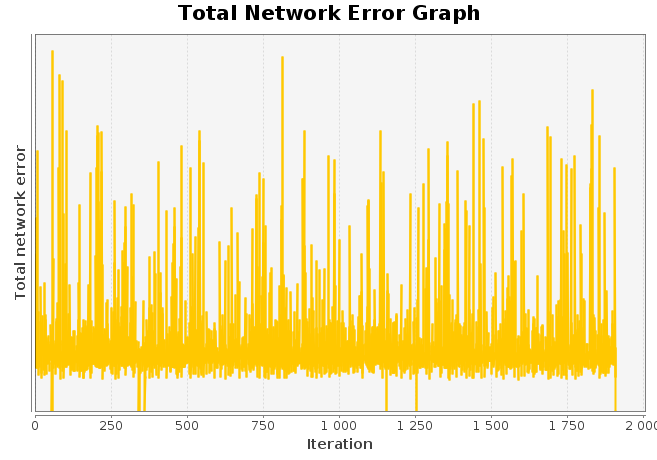
\includegraphics[height=200px]{img/SQUARE_16_704.png}\\
\end{center}

A ce moment, je décide de créer un nouveau dataset calqué sur le second dataset (101) mais contenant tout de même plus d'exemples.
Le dataset 401 : de -2 à 2 avec un pas de 0.01.
Les résultats n'étant pas concluant (pas de convergence avec les réseaux), je décide de créer un dataset, le dataset 101\_2 : de -10 à 10 avec un pas de 0.2.\\
Une fois de plus, le dataset est trop complexe et aucun des perceptron multi-couche n'arrive a converger (testé avec plus de 10000 itération maximum)

\begin{center}
Perceptron multicouche : 1 couche de 16 noeuds.\\
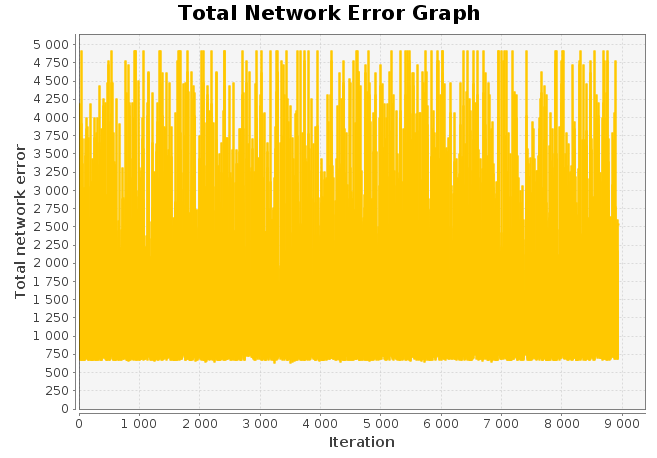
\includegraphics[height=200px]{img/SQUARE_16_101_2.png}\\
Perceptron multicouche : 5 couche de 16 noeuds.\\
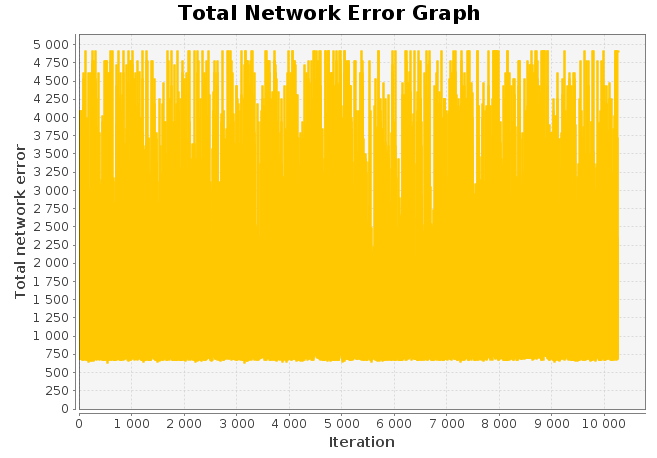
\includegraphics[height=200px]{img/SQUARE_16_16_16_16_16_101_2.png}\\
\end{center}

Une dernière tentative de création de dataset, le dataset 101\_3 : les -100 à 100 avec un pas de 2. Les résultats ne convergent toujours pas, malgré les changements de paramètres d'apprentissages.\\

Pour améliorer mes résultats précédents, je décide de travailler avec le dataset 101 et en changeant les paramètre d'apprentissages afin de trouver de bons paramètres d'apprentissage pour mes 3 réseau retenus.

\begin{center}

\begin{tabular}{|l|c|}
	\hline
	Max Error & 0.001 \\
	\hline
	Learning Rate & 0.2 \\
	\hline
	Momentum & 0.7 \\
	\hline
\end{tabular}

Perceptron multicouche : 1 couche de 8 noeuds.\\
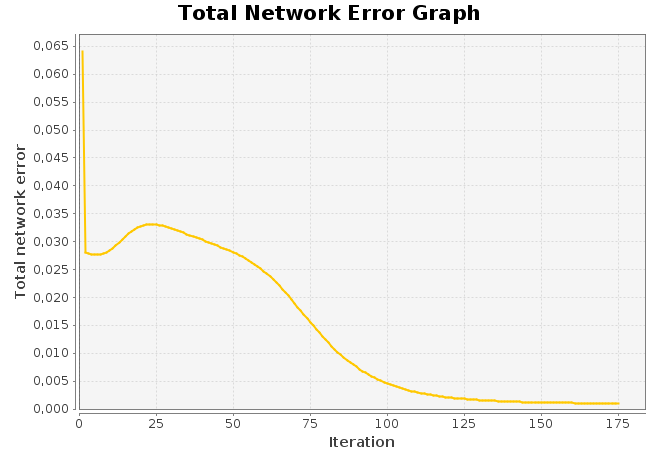
\includegraphics[height=200px]{img/SQUARE_8_101_-3.png}\\
Perceptron multicouche : 1 couche de 16 noeuds.\\
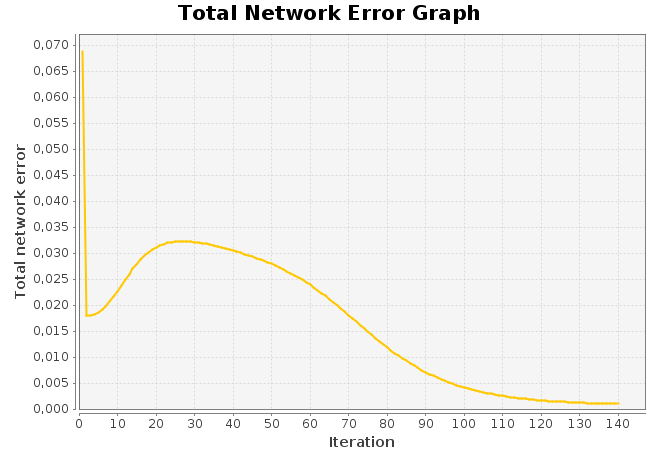
\includegraphics[height=200px]{img/SQUARE_16_101_-3.png}\\
Perceptron multicouche : 2 couche de 16 noeuds.\\
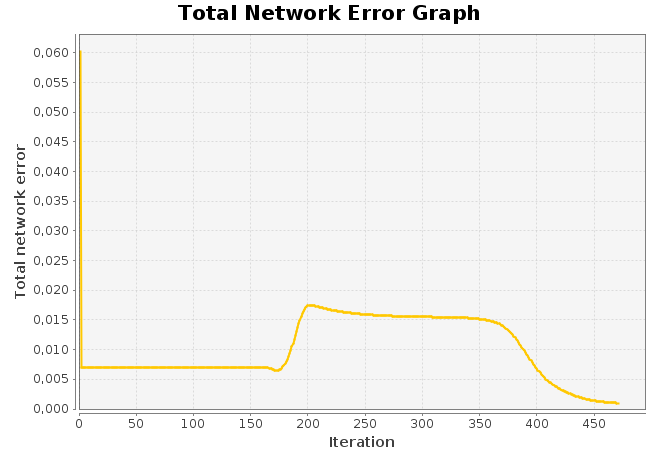
\includegraphics[height=200px]{img/SQUARE_16_16_101_-3.png}\\

\begin{tabular}{|l|c|}
	\hline
	Max Error & 0.0001 \\
	\hline
	Learning Rate & 0.2 \\
	\hline
	Momentum & 0.7 \\
	\hline
\end{tabular}

Perceptron multicouche : 1 couche de 8 noeuds.\\
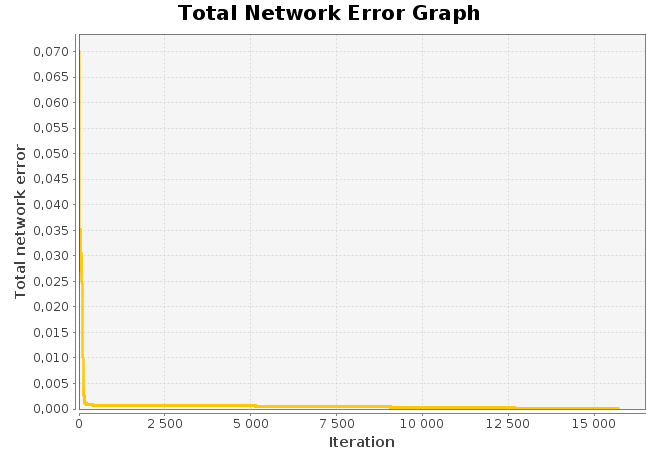
\includegraphics[height=200px]{img/SQUARE_8_101_-4.png}\\
Perceptron multicouche : 1 couche de 16 noeuds.\\
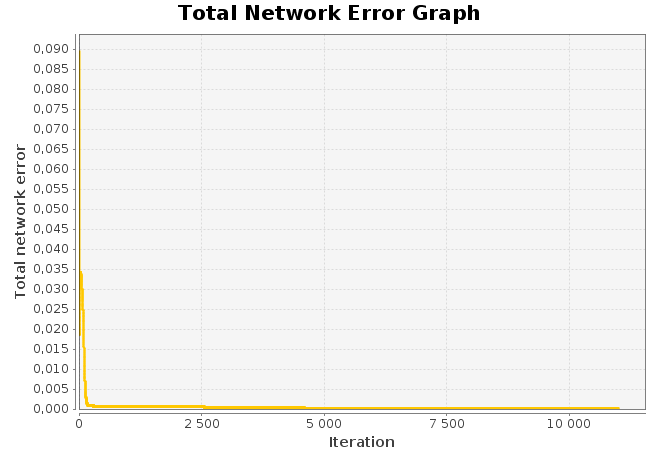
\includegraphics[height=200px]{img/SQUARE_16_101_-4.png}\\
Perceptron multicouche : 2 couche de 16 noeuds.\\
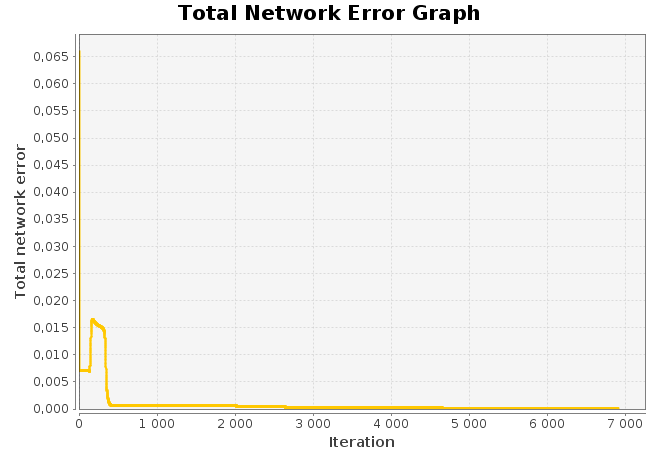
\includegraphics[height=200px]{img/SQUARE_16_16_101_-4.png}\\
\end{center}

A ce moment, on se rend compte que pour une précision supplémentaire, le réseau a 2 couche devient intéressant.

Petite note intéressantes, voici le graph d'erreur d'un perceptron multicouche : 3 couche de 16 noeuds (qui ne converge pas).\\
\begin{center}
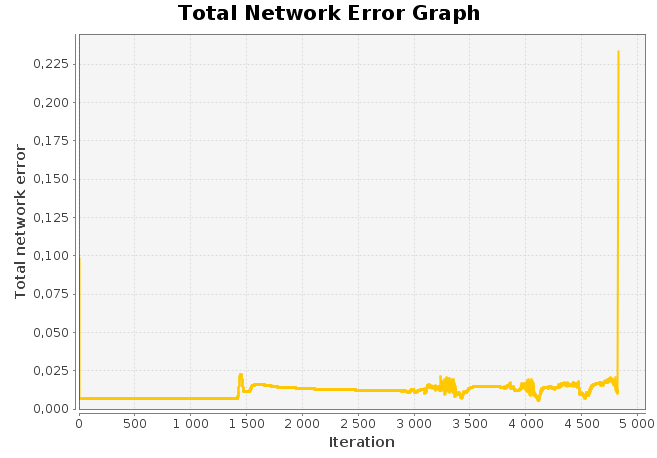
\includegraphics[height=200px]{img/SQUARE_16_16_16_101_-4.png}\\
\end{center}

Pour terminer, nous allons donc nous baser sur ces deux dernier perceptrons multicouche : 1: 1 couches de 16 noeuds et 2: 2 couches de 16 noeuds

\begin{center}
Variation du Learning Rate\\
\begin{tabular}{|l|c|}
	\hline
	Max Error & 0.0001 \\
	\hline
	Learning Rate & 0.02 \\
	\hline
	Momentum & 0.7 \\
	\hline
\end{tabular}

Perceptron multicouche : 1 couche de 16 noeuds.\\
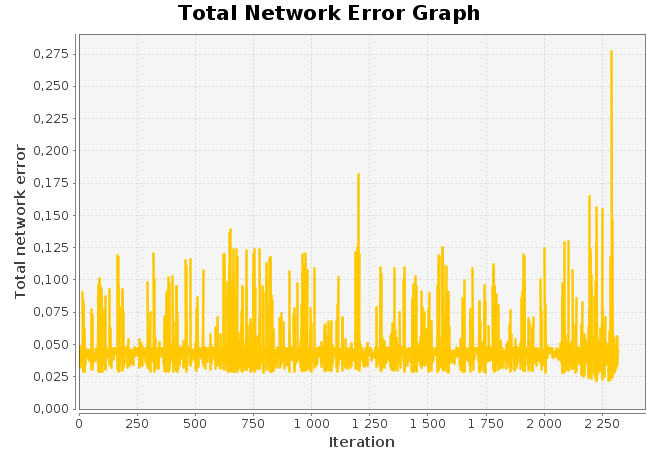
\includegraphics[height=200px]{img/SQUARE_16_101_lr002.png}\\
Perceptron multicouche : 2 couche de 16 noeuds.\\
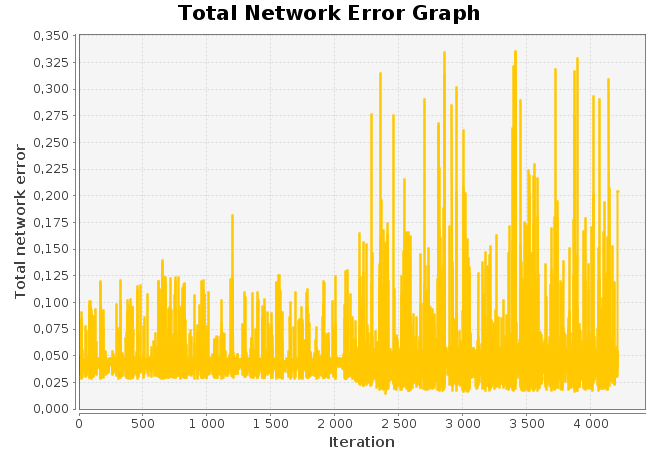
\includegraphics[height=200px]{img/SQUARE_16_16_101_lr002.png}\\

\begin{tabular}{|l|c|}
	\hline
	Max Error & 0.0001 \\
	\hline
	Learning Rate & 2 \\
	\hline
	Momentum & 0.7 \\
	\hline
\end{tabular}

Perceptron multicouche : 2 couche de 16 noeuds.\\
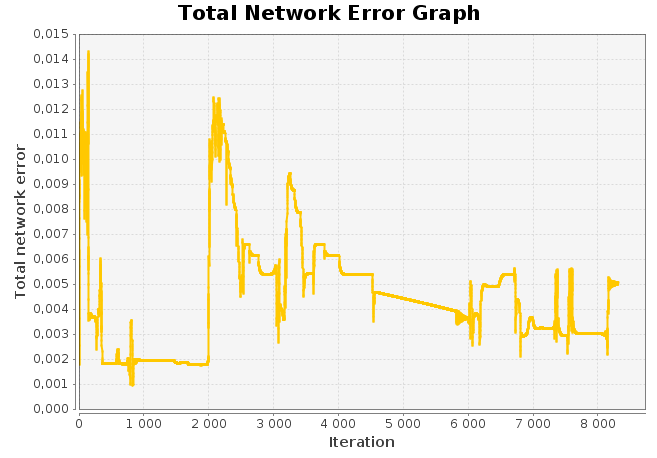
\includegraphics[height=200px]{img/SQUARE_16_101_lr2.png}\\
\end{center}


\begin{center}
Variation du Momentum\\
\begin{tabular}{|l|c|}
	\hline
	Max Error & 0.0001 \\
	\hline
	Learning Rate & 0.2 \\
	\hline
	Momentum & 0.07 \\
	\hline
\end{tabular}

Perceptron multicouche : 2 couche de 16 noeuds.\\
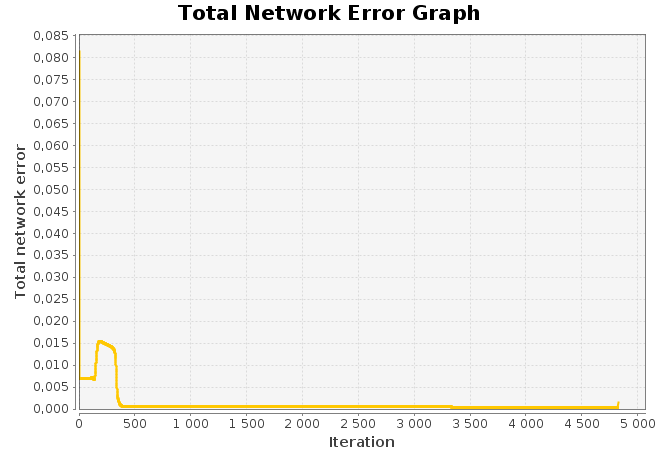
\includegraphics[height=200px]{img/SQUARE_16_16_101_m007.png}\\

\begin{tabular}{|l|c|}
	\hline
	Max Error & 0.0001 \\
	\hline
	Learning Rate & 0.2 \\
	\hline
	Momentum & 7 \\
	\hline
\end{tabular}

Perceptron multicouche : 2 couche de 16 noeuds.\\
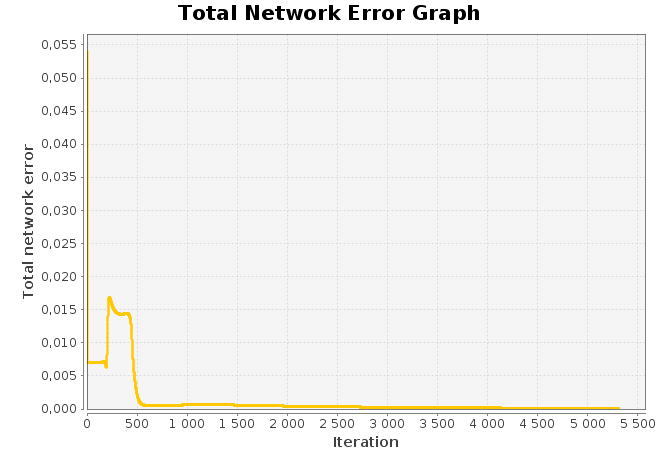
\includegraphics[height=200px]{img/SQUARE_16_16_101_m7.png}\\
\end{center}

\subsubsection{Conclusion}
Le dataset utilisé est très important. Lorsqu'il contient trop peu d'exemple, le réseau peut renvoyer des erreurs basse et pourtant ne pas réellement reproduire les effets demandé. Lorsqu'il contient trop d'exemple, le réseau devient lent, et a tendance a ne pas réussir a converger aussi facilement. Le juste milieu est difficile a trouvé, et dans mon cas, c'est uniquement des tests empirique qui m'ont permit de décider quel dataset utiliser.\\

Finalement, les résultats de mon perceptron multicouche de 2 couche et 16 noeuds sont satisfaisant. 

Mon objectif initiale était d'arriver a faire descendre l'erreur en dessous de 0.0001, et c'est donc une mission accomplie.

La variation de tous les paramètres est importante, malheureusement il n'existe pas de règles ou de guide a suivre pour créer un bon réseau de neurones.

De nombreux tests effectués n'apparaissent pas dans ce rapport (faute de bon résultats) mais les 19 réseaux de neurones et les 10 ensemble de test sont disponibles dans le projet neuroph si nécessaire.

\chapter{Annexes}
\section{NeurophStudio}
\subsection{Reset / Randomize}

\end{document}